% Options for packages loaded elsewhere
\PassOptionsToPackage{unicode}{hyperref}
\PassOptionsToPackage{hyphens}{url}
\PassOptionsToPackage{dvipsnames,svgnames,x11names}{xcolor}
%
\documentclass[
  letterpaper,
]{article}

\usepackage{amsmath,amssymb}
\usepackage{setspace}
\usepackage{iftex}
\ifPDFTeX
  \usepackage[T1]{fontenc}
  \usepackage[utf8]{inputenc}
  \usepackage{textcomp} % provide euro and other symbols
\else % if luatex or xetex
  \usepackage{unicode-math}
  \defaultfontfeatures{Scale=MatchLowercase}
  \defaultfontfeatures[\rmfamily]{Ligatures=TeX,Scale=1}
\fi
\usepackage{lmodern}
\ifPDFTeX\else  
    % xetex/luatex font selection
\fi
% Use upquote if available, for straight quotes in verbatim environments
\IfFileExists{upquote.sty}{\usepackage{upquote}}{}
\IfFileExists{microtype.sty}{% use microtype if available
  \usepackage[]{microtype}
  \UseMicrotypeSet[protrusion]{basicmath} % disable protrusion for tt fonts
}{}
\usepackage{xcolor}
\usepackage[top=2.54cm,right=2.54cm,bottom=2.54cm,left=2.54cm]{geometry}
\setlength{\emergencystretch}{3em} % prevent overfull lines
\setcounter{secnumdepth}{3}
% Make \paragraph and \subparagraph free-standing
\makeatletter
\ifx\paragraph\undefined\else
  \let\oldparagraph\paragraph
  \renewcommand{\paragraph}{
    \@ifstar
      \xxxParagraphStar
      \xxxParagraphNoStar
  }
  \newcommand{\xxxParagraphStar}[1]{\oldparagraph*{#1}\mbox{}}
  \newcommand{\xxxParagraphNoStar}[1]{\oldparagraph{#1}\mbox{}}
\fi
\ifx\subparagraph\undefined\else
  \let\oldsubparagraph\subparagraph
  \renewcommand{\subparagraph}{
    \@ifstar
      \xxxSubParagraphStar
      \xxxSubParagraphNoStar
  }
  \newcommand{\xxxSubParagraphStar}[1]{\oldsubparagraph*{#1}\mbox{}}
  \newcommand{\xxxSubParagraphNoStar}[1]{\oldsubparagraph{#1}\mbox{}}
\fi
\makeatother

\usepackage{color}
\usepackage{fancyvrb}
\newcommand{\VerbBar}{|}
\newcommand{\VERB}{\Verb[commandchars=\\\{\}]}
\DefineVerbatimEnvironment{Highlighting}{Verbatim}{commandchars=\\\{\}}
% Add ',fontsize=\small' for more characters per line
\usepackage{framed}
\definecolor{shadecolor}{RGB}{241,243,245}
\newenvironment{Shaded}{\begin{snugshade}}{\end{snugshade}}
\newcommand{\AlertTok}[1]{\textcolor[rgb]{0.68,0.00,0.00}{#1}}
\newcommand{\AnnotationTok}[1]{\textcolor[rgb]{0.37,0.37,0.37}{#1}}
\newcommand{\AttributeTok}[1]{\textcolor[rgb]{0.40,0.45,0.13}{#1}}
\newcommand{\BaseNTok}[1]{\textcolor[rgb]{0.68,0.00,0.00}{#1}}
\newcommand{\BuiltInTok}[1]{\textcolor[rgb]{0.00,0.23,0.31}{#1}}
\newcommand{\CharTok}[1]{\textcolor[rgb]{0.13,0.47,0.30}{#1}}
\newcommand{\CommentTok}[1]{\textcolor[rgb]{0.37,0.37,0.37}{#1}}
\newcommand{\CommentVarTok}[1]{\textcolor[rgb]{0.37,0.37,0.37}{\textit{#1}}}
\newcommand{\ConstantTok}[1]{\textcolor[rgb]{0.56,0.35,0.01}{#1}}
\newcommand{\ControlFlowTok}[1]{\textcolor[rgb]{0.00,0.23,0.31}{\textbf{#1}}}
\newcommand{\DataTypeTok}[1]{\textcolor[rgb]{0.68,0.00,0.00}{#1}}
\newcommand{\DecValTok}[1]{\textcolor[rgb]{0.68,0.00,0.00}{#1}}
\newcommand{\DocumentationTok}[1]{\textcolor[rgb]{0.37,0.37,0.37}{\textit{#1}}}
\newcommand{\ErrorTok}[1]{\textcolor[rgb]{0.68,0.00,0.00}{#1}}
\newcommand{\ExtensionTok}[1]{\textcolor[rgb]{0.00,0.23,0.31}{#1}}
\newcommand{\FloatTok}[1]{\textcolor[rgb]{0.68,0.00,0.00}{#1}}
\newcommand{\FunctionTok}[1]{\textcolor[rgb]{0.28,0.35,0.67}{#1}}
\newcommand{\ImportTok}[1]{\textcolor[rgb]{0.00,0.46,0.62}{#1}}
\newcommand{\InformationTok}[1]{\textcolor[rgb]{0.37,0.37,0.37}{#1}}
\newcommand{\KeywordTok}[1]{\textcolor[rgb]{0.00,0.23,0.31}{\textbf{#1}}}
\newcommand{\NormalTok}[1]{\textcolor[rgb]{0.00,0.23,0.31}{#1}}
\newcommand{\OperatorTok}[1]{\textcolor[rgb]{0.37,0.37,0.37}{#1}}
\newcommand{\OtherTok}[1]{\textcolor[rgb]{0.00,0.23,0.31}{#1}}
\newcommand{\PreprocessorTok}[1]{\textcolor[rgb]{0.68,0.00,0.00}{#1}}
\newcommand{\RegionMarkerTok}[1]{\textcolor[rgb]{0.00,0.23,0.31}{#1}}
\newcommand{\SpecialCharTok}[1]{\textcolor[rgb]{0.37,0.37,0.37}{#1}}
\newcommand{\SpecialStringTok}[1]{\textcolor[rgb]{0.13,0.47,0.30}{#1}}
\newcommand{\StringTok}[1]{\textcolor[rgb]{0.13,0.47,0.30}{#1}}
\newcommand{\VariableTok}[1]{\textcolor[rgb]{0.07,0.07,0.07}{#1}}
\newcommand{\VerbatimStringTok}[1]{\textcolor[rgb]{0.13,0.47,0.30}{#1}}
\newcommand{\WarningTok}[1]{\textcolor[rgb]{0.37,0.37,0.37}{\textit{#1}}}

\providecommand{\tightlist}{%
  \setlength{\itemsep}{0pt}\setlength{\parskip}{0pt}}\usepackage{longtable,booktabs,array}
\usepackage{calc} % for calculating minipage widths
% Correct order of tables after \paragraph or \subparagraph
\usepackage{etoolbox}
\makeatletter
\patchcmd\longtable{\par}{\if@noskipsec\mbox{}\fi\par}{}{}
\makeatother
% Allow footnotes in longtable head/foot
\IfFileExists{footnotehyper.sty}{\usepackage{footnotehyper}}{\usepackage{footnote}}
\makesavenoteenv{longtable}
\usepackage{graphicx}
\makeatletter
\def\maxwidth{\ifdim\Gin@nat@width>\linewidth\linewidth\else\Gin@nat@width\fi}
\def\maxheight{\ifdim\Gin@nat@height>\textheight\textheight\else\Gin@nat@height\fi}
\makeatother
% Scale images if necessary, so that they will not overflow the page
% margins by default, and it is still possible to overwrite the defaults
% using explicit options in \includegraphics[width, height, ...]{}
\setkeys{Gin}{width=\maxwidth,height=\maxheight,keepaspectratio}
% Set default figure placement to htbp
\makeatletter
\def\fps@figure{htbp}
\makeatother

\makeatletter
\@ifpackageloaded{caption}{}{\usepackage{caption}}
\AtBeginDocument{%
\ifdefined\contentsname
  \renewcommand*\contentsname{Table of contents}
\else
  \newcommand\contentsname{Table of contents}
\fi
\ifdefined\listfigurename
  \renewcommand*\listfigurename{List of Figures}
\else
  \newcommand\listfigurename{List of Figures}
\fi
\ifdefined\listtablename
  \renewcommand*\listtablename{List of Tables}
\else
  \newcommand\listtablename{List of Tables}
\fi
\ifdefined\figurename
  \renewcommand*\figurename{Figure}
\else
  \newcommand\figurename{Figure}
\fi
\ifdefined\tablename
  \renewcommand*\tablename{Table}
\else
  \newcommand\tablename{Table}
\fi
}
\@ifpackageloaded{float}{}{\usepackage{float}}
\floatstyle{ruled}
\@ifundefined{c@chapter}{\newfloat{codelisting}{h}{lop}}{\newfloat{codelisting}{h}{lop}[chapter]}
\floatname{codelisting}{Listing}
\newcommand*\listoflistings{\listof{codelisting}{List of Listings}}
\makeatother
\makeatletter
\makeatother
\makeatletter
\@ifpackageloaded{caption}{}{\usepackage{caption}}
\@ifpackageloaded{subcaption}{}{\usepackage{subcaption}}
\makeatother

\ifLuaTeX
  \usepackage{selnolig}  % disable illegal ligatures
\fi
\usepackage{bookmark}

\IfFileExists{xurl.sty}{\usepackage{xurl}}{} % add URL line breaks if available
\urlstyle{same} % disable monospaced font for URLs
% Make links footnotes instead of hotlinks:
\DeclareRobustCommand{\href}[2]{#2\footnote{\url{#1}}}
\hypersetup{
  pdftitle={Choosing colors and shapes in ggplot2},
  pdfauthor={Simone Santoni},
  colorlinks=true,
  linkcolor={blue},
  filecolor={Maroon},
  citecolor={Blue},
  urlcolor={Blue},
  pdfcreator={LaTeX via pandoc}}


\title{Choosing colors and shapes in ggplot2}
\author{Simone Santoni}
\date{2024-10-31}

\begin{document}
\maketitle
\begin{abstract}
This notebook illustrates how to change
\end{abstract}


\setstretch{1.1}
\section{Notebook setup}\label{notebook-setup}

\subsection{Load libraries}\label{load-libraries}

\begin{Shaded}
\begin{Highlighting}[]
\FunctionTok{library}\NormalTok{(ggplot2)}
\FunctionTok{library}\NormalTok{(dplyr)}
\end{Highlighting}
\end{Shaded}

\begin{verbatim}

Attaching package: 'dplyr'
\end{verbatim}

\begin{verbatim}
The following objects are masked from 'package:stats':

    filter, lag
\end{verbatim}

\begin{verbatim}
The following objects are masked from 'package:base':

    intersect, setdiff, setequal, union
\end{verbatim}

\begin{Shaded}
\begin{Highlighting}[]
\FunctionTok{library}\NormalTok{(readr)}
\end{Highlighting}
\end{Shaded}

\subsection{Load data}\label{load-data}

The toy dataset we'll use in this notebook is
\texttt{laptop\_price.csv}. It contains information on the price of
laptops, as well as the laptops' core featurs. The source for the
dataset is https://www.kaggle.com/datasets/muhammetvarl/laptop-price

\begin{Shaded}
\begin{Highlighting}[]
\NormalTok{df }\OtherTok{\textless{}{-}} \FunctionTok{read\_csv}\NormalTok{(}\StringTok{"\textasciitilde{}/githubRepos/data{-}viz{-}smm635/data/laptops/laptop\_price.csv"}\NormalTok{)}
\end{Highlighting}
\end{Shaded}

\begin{verbatim}
Rows: 1303 Columns: 13
-- Column specification --------------------------------------------------------
Delimiter: ","
chr (10): Company, Product, TypeName, ScreenResolution, Cpu, Ram, Memory, Gp...
dbl  (3): laptop_ID, Inches, Price_euros

i Use `spec()` to retrieve the full column specification for this data.
i Specify the column types or set `show_col_types = FALSE` to quiet this message.
\end{verbatim}

\begin{Shaded}
\begin{Highlighting}[]
\NormalTok{df}
\end{Highlighting}
\end{Shaded}

\begin{verbatim}
# A tibble: 1,303 x 13
   laptop_ID Company Product TypeName Inches ScreenResolution Cpu   Ram   Memory
       <dbl> <chr>   <chr>   <chr>     <dbl> <chr>            <chr> <chr> <chr> 
 1         1 Apple   MacBoo~ Ultrabo~   13.3 IPS Panel Retin~ Inte~ 8GB   128GB~
 2         2 Apple   Macboo~ Ultrabo~   13.3 1440x900         Inte~ 8GB   128GB~
 3         3 HP      250 G6  Notebook   15.6 Full HD 1920x10~ Inte~ 8GB   256GB~
 4         4 Apple   MacBoo~ Ultrabo~   15.4 IPS Panel Retin~ Inte~ 16GB  512GB~
 5         5 Apple   MacBoo~ Ultrabo~   13.3 IPS Panel Retin~ Inte~ 8GB   256GB~
 6         6 Acer    Aspire~ Notebook   15.6 1366x768         AMD ~ 4GB   500GB~
 7         7 Apple   MacBoo~ Ultrabo~   15.4 IPS Panel Retin~ Inte~ 16GB  256GB~
 8         8 Apple   Macboo~ Ultrabo~   13.3 1440x900         Inte~ 8GB   256GB~
 9         9 Asus    ZenBoo~ Ultrabo~   14   Full HD 1920x10~ Inte~ 16GB  512GB~
10        10 Acer    Swift 3 Ultrabo~   14   IPS Panel Full ~ Inte~ 8GB   256GB~
# i 1,293 more rows
# i 4 more variables: Gpu <chr>, OpSys <chr>, Weight <chr>, Price_euros <dbl>
\end{verbatim}

\section{Colors}\label{colors}

\subsection{Visual forms' inner color, boarder color, and
transparency}\label{visual-forms-inner-color-boarder-color-and-transparency}

In \texttt{ggplot2}, it is possible to alter a visual form's default
color by passing an optional parameter to the geomtric object at hand.
Let's consider a bar chart showing the distribution of laptops across
different screen sizes. Figure~\ref{fig-base} illustrates a chart whose
bars exhibit \texttt{ggplot2}'s default color. Populating the optional
parameter \texttt{fill} would alter the chosen visual form's inner color
-- see Figure~\ref{fig-fill}; the optional parameter \texttt{colour}
affects the visual form's boarder color -- see
Figure~\ref{fig-fillandboard}. It is also possible to regulate the
transparency of the chosen color by fixing the optional \texttt{alpha}
parameter -- see Figure~\ref{fig-alpha}. Note that the smaller is the
scalar value you pass to \texttt{alpha}, the more transparent is the
visual form -- see Figure~\ref{fig-alphaagg}.

\begin{Shaded}
\begin{Highlighting}[]
\NormalTok{p }\OtherTok{\textless{}{-}} \FunctionTok{ggplot}\NormalTok{(}\AttributeTok{data =}\NormalTok{ df, }\AttributeTok{mapping =} \FunctionTok{aes}\NormalTok{(}\FunctionTok{factor}\NormalTok{(Inches)))}
\NormalTok{p }\SpecialCharTok{+} \FunctionTok{geom\_bar}\NormalTok{()}
\end{Highlighting}
\end{Shaded}

\begin{figure}[H]

\centering{

\pandocbounded{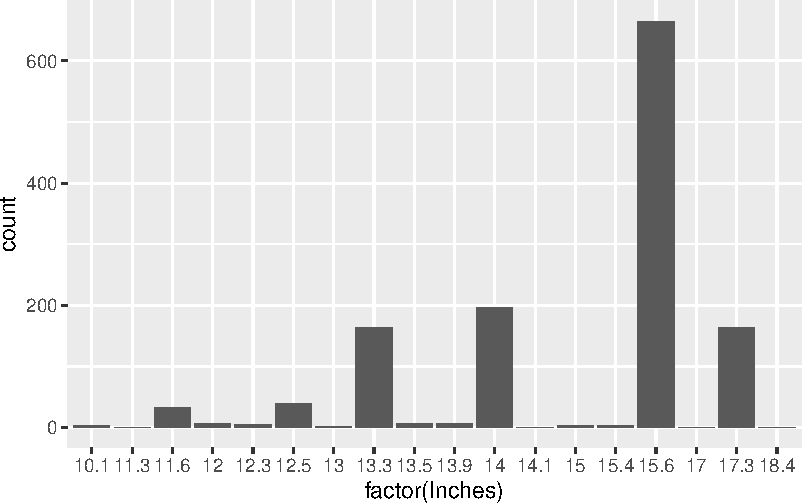
\includegraphics[keepaspectratio]{color_and_shapes_files/figure-pdf/fig-base-1.pdf}}

}

\caption{\label{fig-base}A bar chart with default colors}

\end{figure}%

\begin{Shaded}
\begin{Highlighting}[]
\NormalTok{p }\OtherTok{\textless{}{-}} \FunctionTok{ggplot}\NormalTok{(}\AttributeTok{data =}\NormalTok{ df, }\AttributeTok{mapping =} \FunctionTok{aes}\NormalTok{(}\FunctionTok{factor}\NormalTok{(Inches)))}
\NormalTok{p }\SpecialCharTok{+} \FunctionTok{geom\_bar}\NormalTok{(}\AttributeTok{fill =} \StringTok{"magenta"}\NormalTok{)}
\end{Highlighting}
\end{Shaded}

\begin{figure}[H]

\centering{

\pandocbounded{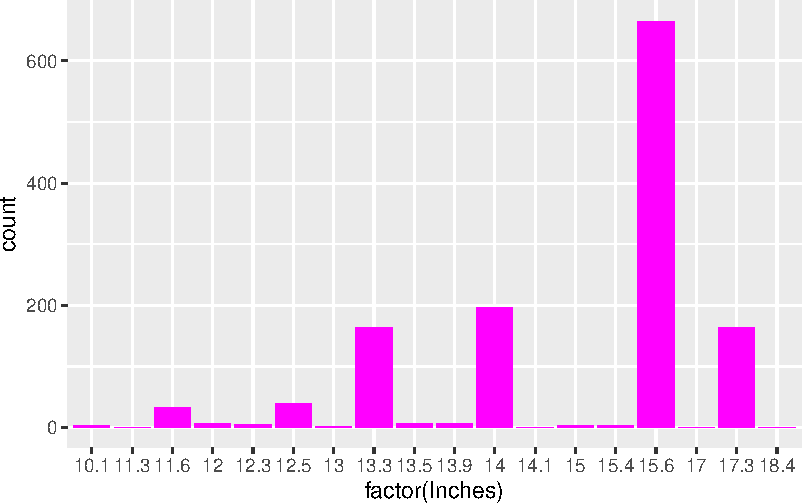
\includegraphics[keepaspectratio]{color_and_shapes_files/figure-pdf/fig-fill-1.pdf}}

}

\caption{\label{fig-fill}A bar chart with custom fill color}

\end{figure}%

\begin{Shaded}
\begin{Highlighting}[]
\NormalTok{p }\OtherTok{\textless{}{-}} \FunctionTok{ggplot}\NormalTok{(}\AttributeTok{data =}\NormalTok{ df, }\AttributeTok{mapping =} \FunctionTok{aes}\NormalTok{(}\FunctionTok{factor}\NormalTok{(Inches)))}
\NormalTok{p }\SpecialCharTok{+} \FunctionTok{geom\_bar}\NormalTok{(}\AttributeTok{fill =} \StringTok{"magenta"}\NormalTok{, }\AttributeTok{colour =} \StringTok{"blue"}\NormalTok{)}
\end{Highlighting}
\end{Shaded}

\begin{figure}[H]

\centering{

\pandocbounded{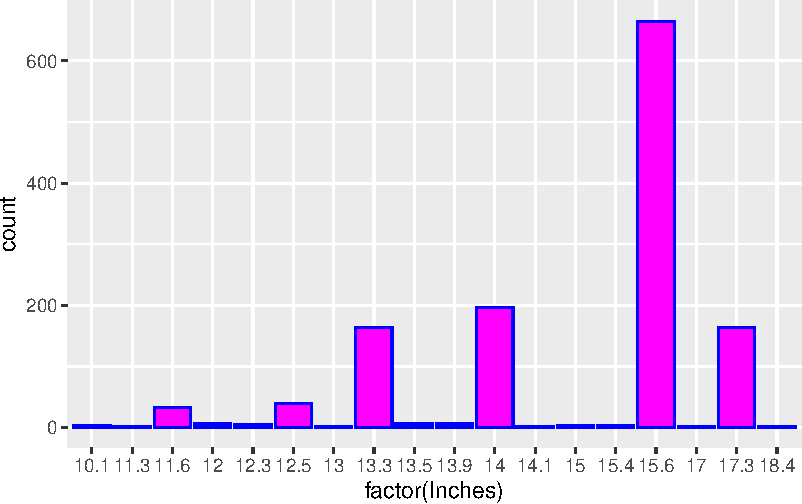
\includegraphics[keepaspectratio]{color_and_shapes_files/figure-pdf/fig-fillandboard-1.pdf}}

}

\caption{\label{fig-fillandboard}A bar chart with custom fill and
boarder color}

\end{figure}%

\begin{Shaded}
\begin{Highlighting}[]
\NormalTok{p }\OtherTok{\textless{}{-}} \FunctionTok{ggplot}\NormalTok{(}\AttributeTok{data =}\NormalTok{ df, }\AttributeTok{mapping =} \FunctionTok{aes}\NormalTok{(}\FunctionTok{factor}\NormalTok{(Inches)))}
\NormalTok{p }\SpecialCharTok{+} \FunctionTok{geom\_bar}\NormalTok{(}\AttributeTok{fill =} \StringTok{"green"}\NormalTok{, }\AttributeTok{alpha =} \FloatTok{0.5}\NormalTok{)}
\end{Highlighting}
\end{Shaded}

\begin{figure}[H]

\centering{

\pandocbounded{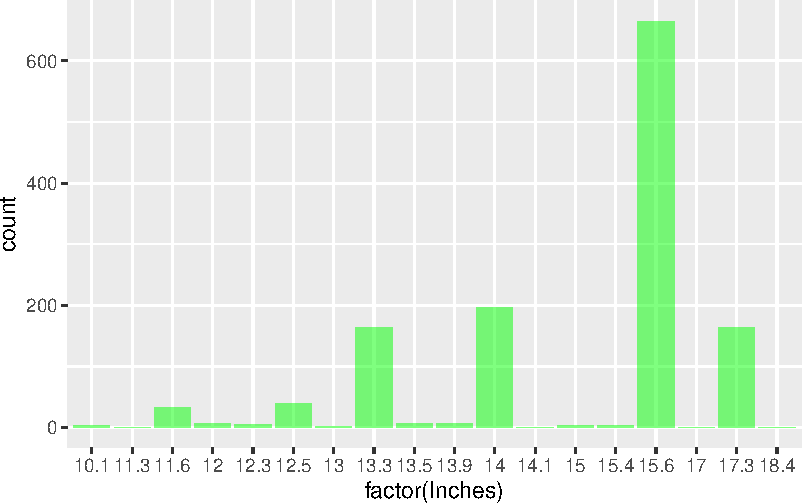
\includegraphics[keepaspectratio]{color_and_shapes_files/figure-pdf/fig-alpha-1.pdf}}

}

\caption{\label{fig-alpha}A bar chart with adjusted color transparency}

\end{figure}%

\begin{Shaded}
\begin{Highlighting}[]
\NormalTok{p }\OtherTok{\textless{}{-}} \FunctionTok{ggplot}\NormalTok{(}\AttributeTok{data =}\NormalTok{ df, }\AttributeTok{mapping =} \FunctionTok{aes}\NormalTok{(}\FunctionTok{factor}\NormalTok{(Inches)))}
\NormalTok{p }\SpecialCharTok{+} \FunctionTok{geom\_bar}\NormalTok{(}\AttributeTok{fill =} \StringTok{"green"}\NormalTok{, }\AttributeTok{alpha =} \FloatTok{0.1}\NormalTok{)}
\end{Highlighting}
\end{Shaded}

\begin{figure}[H]

\centering{

\pandocbounded{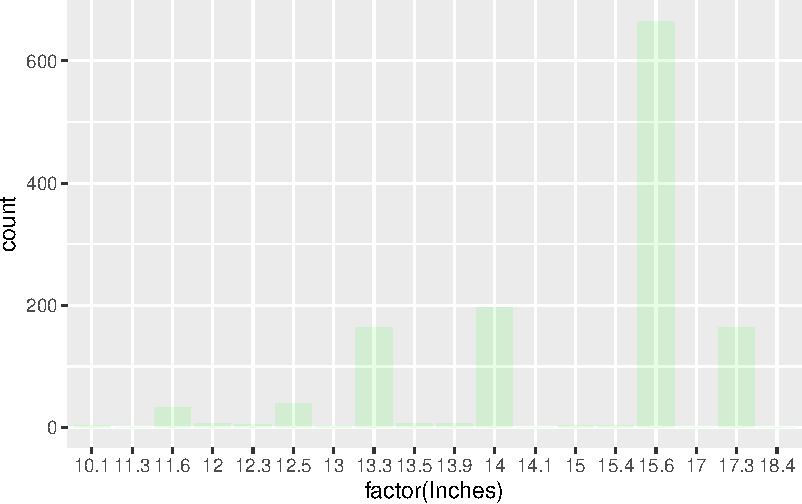
\includegraphics[keepaspectratio]{color_and_shapes_files/figure-pdf/fig-alphaagg-1.pdf}}

}

\caption{\label{fig-alphaagg}A bar chart with alpha = 0.1}

\end{figure}%

\subsection{Scales}\label{scales}

\texttt{ggplot2} comes with plenty of
\href{https://ggplot2-book.org/scales-colour\#brewer-scales}{color
scales and palettes} that can help discriminate visually various data
groups. Let's suppose to expand on the visualization reported in
Figure~\ref{fig-boxplot}, dealing with the distribution of laptop price
across different screen size groups. Specifically, we want to add
another dimension to Figure~\ref{fig-boxplot} to show how laptop prices
change across screen and ram size groups. By default, \texttt{ggplot2}
will use the \texttt{hue} color scale see ―
Figure~\ref{fig-boxplotdefault}. To adopt a non-default color scale, the
optional argument \texttt{scale\_color\_*} must be populated. In
Figure~\ref{fig-boxplotbrewer}, I adopt a color scale for discrete data,
namely
\href{https://ggplot2-book.org/scales-colour\#brewer-scales}{\texttt{brewer}}.
\emph{Warning}: always ensure to pair discrete (continuous) color scales
with discrete (continuous) variables. Otherwise, \texttt{ggplot2} will
return an error, e.g.,
\texttt{Discrete\ values\ supplied\ to\ continuous\ scale}.

\begin{Shaded}
\begin{Highlighting}[]
\NormalTok{p }\OtherTok{\textless{}{-}} \FunctionTok{ggplot}\NormalTok{(}\AttributeTok{data =}\NormalTok{ df, }\AttributeTok{mapping =} \FunctionTok{aes}\NormalTok{(}\AttributeTok{x =} \FunctionTok{factor}\NormalTok{(Inches), }\AttributeTok{y =}\NormalTok{ Price\_euros))}
\NormalTok{p }\SpecialCharTok{+} \FunctionTok{geom\_boxplot}\NormalTok{()}
\end{Highlighting}
\end{Shaded}

\begin{figure}[H]

\centering{

\pandocbounded{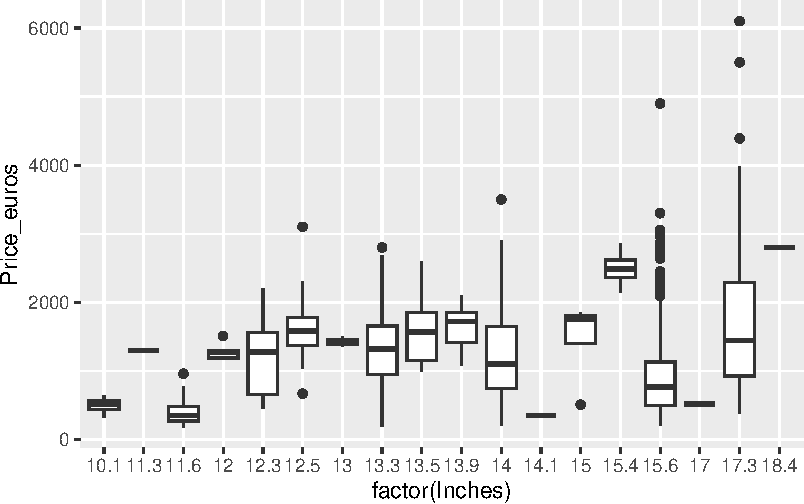
\includegraphics[keepaspectratio]{color_and_shapes_files/figure-pdf/fig-boxplot-1.pdf}}

}

\caption{\label{fig-boxplot}Distribution of laptop prices by scree size
group}

\end{figure}%

\begin{Shaded}
\begin{Highlighting}[]
\NormalTok{p }\OtherTok{\textless{}{-}} \FunctionTok{ggplot}\NormalTok{(}\AttributeTok{data =}\NormalTok{ df, }\AttributeTok{mapping =} \FunctionTok{aes}\NormalTok{(}\AttributeTok{x =} \FunctionTok{factor}\NormalTok{(Inches), }\AttributeTok{y =}\NormalTok{ Price\_euros))}
\NormalTok{p }\SpecialCharTok{+} \FunctionTok{geom\_boxplot}\NormalTok{(}\FunctionTok{aes}\NormalTok{(}\AttributeTok{colour =}\NormalTok{ Ram))}
\end{Highlighting}
\end{Shaded}

\begin{figure}[H]

\centering{

\pandocbounded{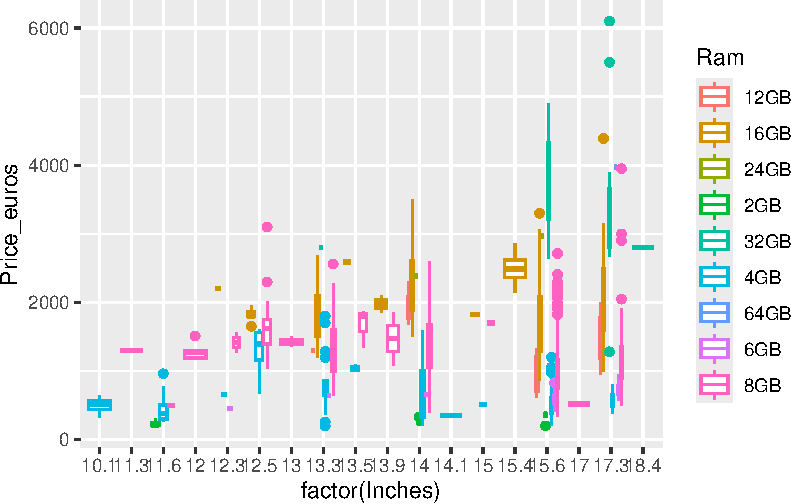
\includegraphics[keepaspectratio]{color_and_shapes_files/figure-pdf/fig-boxplotdefault-1.pdf}}

}

\caption{\label{fig-boxplotdefault}}

\end{figure}%

\begin{Shaded}
\begin{Highlighting}[]
\NormalTok{p }\OtherTok{\textless{}{-}} \FunctionTok{ggplot}\NormalTok{(}\AttributeTok{data =}\NormalTok{ df, }\AttributeTok{mapping =} \FunctionTok{aes}\NormalTok{(}\AttributeTok{x =} \FunctionTok{factor}\NormalTok{(Inches), }\AttributeTok{y =}\NormalTok{ Price\_euros))}
\NormalTok{p }\SpecialCharTok{+} \FunctionTok{geom\_boxplot}\NormalTok{(}\FunctionTok{aes}\NormalTok{(}\AttributeTok{colour =}\NormalTok{ Ram)) }\SpecialCharTok{+} \FunctionTok{scale\_color\_brewer}\NormalTok{(}\AttributeTok{palette =} \StringTok{"Paired"}\NormalTok{)}
\end{Highlighting}
\end{Shaded}

\begin{figure}[H]

\centering{

\pandocbounded{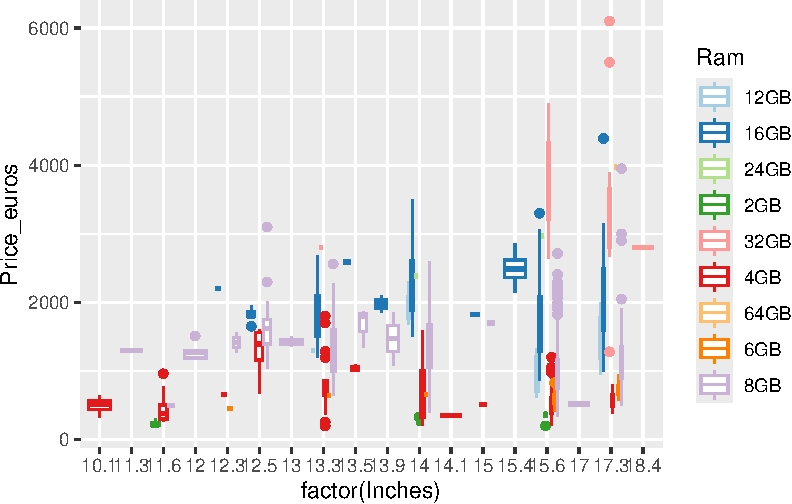
\includegraphics[keepaspectratio]{color_and_shapes_files/figure-pdf/fig-boxplotbrewer-1.pdf}}

}

\caption{\label{fig-boxplotbrewer}}

\end{figure}%

\section{Shapes}\label{shapes}

In data visualization, shapes can play a role similar to colors, by
representing further data dimensions. For example,
Figure~\ref{fig-colors} and Figure~\ref{fig-shapes} use color and
shapes, respectively, to denote two different data series regarding
Apple and Lenovo laptops.

\begin{Shaded}
\begin{Highlighting}[]
\NormalTok{cols }\OtherTok{\textless{}{-}} \FunctionTok{c}\NormalTok{(}\StringTok{"Company"}\NormalTok{, }\StringTok{"Inches"}\NormalTok{)}
\NormalTok{apple\_lenovo }\OtherTok{\textless{}{-}}\NormalTok{ df }\SpecialCharTok{|\textgreater{}} \FunctionTok{filter}\NormalTok{(Company }\SpecialCharTok{==} \StringTok{"Apple"} \SpecialCharTok{|}\NormalTok{ Company }\SpecialCharTok{==} \StringTok{"Lenovo"}\NormalTok{)}
\NormalTok{ave }\OtherTok{\textless{}{-}}\NormalTok{ apple\_lenovo }\SpecialCharTok{|\textgreater{}} \FunctionTok{group\_by}\NormalTok{(}\FunctionTok{across}\NormalTok{(}\FunctionTok{all\_of}\NormalTok{(cols))) }\SpecialCharTok{|\textgreater{}} \FunctionTok{summarize}\NormalTok{(}\AttributeTok{ave\_price =} \FunctionTok{mean}\NormalTok{(Price\_euros))}
\end{Highlighting}
\end{Shaded}

\begin{verbatim}
`summarise()` has grouped output by 'Company'. You can override using the
`.groups` argument.
\end{verbatim}

\begin{Shaded}
\begin{Highlighting}[]
\NormalTok{p }\OtherTok{\textless{}{-}} \FunctionTok{ggplot}\NormalTok{(}\AttributeTok{data =}\NormalTok{ ave, }\AttributeTok{mapping =} \FunctionTok{aes}\NormalTok{(}\AttributeTok{x =} \FunctionTok{factor}\NormalTok{(Inches), }\AttributeTok{y =}\NormalTok{ ave\_price, }\AttributeTok{color =} \FunctionTok{factor}\NormalTok{(Company)))}
\NormalTok{p }\SpecialCharTok{+} \FunctionTok{geom\_point}\NormalTok{()}
\end{Highlighting}
\end{Shaded}

\begin{figure}[H]

\centering{

\pandocbounded{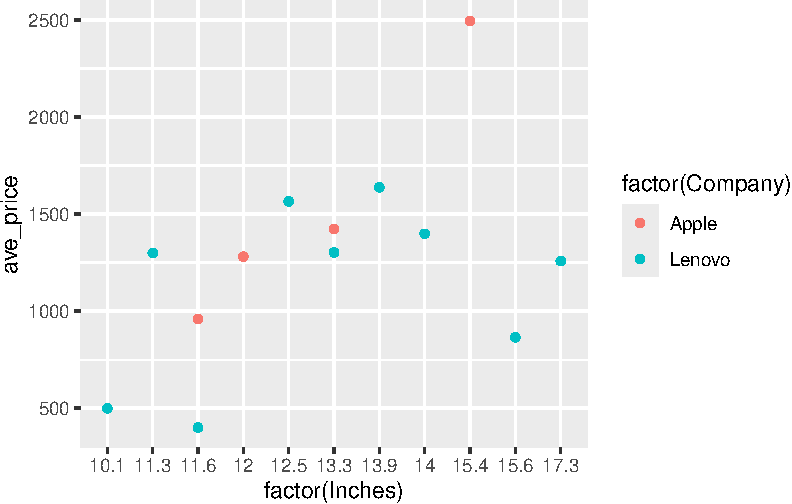
\includegraphics[keepaspectratio]{color_and_shapes_files/figure-pdf/fig-colors-1.pdf}}

}

\caption{\label{fig-colors}Colors denote companie}

\end{figure}%

\begin{Shaded}
\begin{Highlighting}[]
\NormalTok{p }\OtherTok{\textless{}{-}} \FunctionTok{ggplot}\NormalTok{(}\AttributeTok{data =}\NormalTok{ ave, }\AttributeTok{mapping =} \FunctionTok{aes}\NormalTok{(}\AttributeTok{x =} \FunctionTok{factor}\NormalTok{(Inches), }\AttributeTok{y =}\NormalTok{ ave\_price, }\AttributeTok{shape =} \FunctionTok{factor}\NormalTok{(Company)))}
\NormalTok{p }\SpecialCharTok{+} \FunctionTok{geom\_point}\NormalTok{()}
\end{Highlighting}
\end{Shaded}

\begin{figure}[H]

\centering{

\pandocbounded{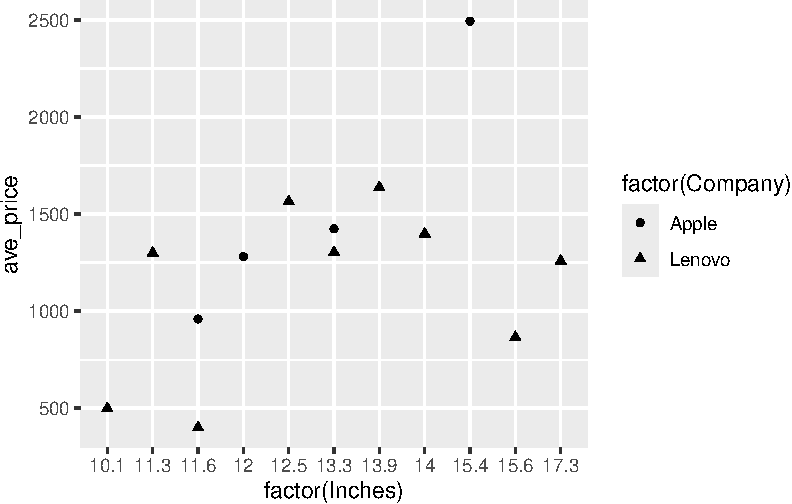
\includegraphics[keepaspectratio]{color_and_shapes_files/figure-pdf/fig-shapes-1.pdf}}

}

\caption{\label{fig-shapes}Shapes denote companies}

\end{figure}%

At the same time, one may want to adopt a non-default shape across all
data series. That would be the case of Figure~\ref{fig-changingshapes},
in which shape `5' ― an empty circle ― replaces \texttt{ggplot2}'s
default shape. \textbf{?@fig-ggplot2shapes} provides a summary of the
shapes available in \texttt{ggplot2} and their underlying numeric codes.

\begin{Shaded}
\begin{Highlighting}[]
\NormalTok{p }\OtherTok{\textless{}{-}} \FunctionTok{ggplot}\NormalTok{(}\AttributeTok{data =}\NormalTok{ ave, }\AttributeTok{mapping =} \FunctionTok{aes}\NormalTok{(}\AttributeTok{x =} \FunctionTok{factor}\NormalTok{(Inches), }\AttributeTok{y =}\NormalTok{ ave\_price, }\AttributeTok{color =} \FunctionTok{factor}\NormalTok{(Company)))}
\NormalTok{p }\SpecialCharTok{+} \FunctionTok{geom\_point}\NormalTok{(}\AttributeTok{shape =} \DecValTok{5}\NormalTok{)}
\end{Highlighting}
\end{Shaded}

\begin{figure}[H]

\centering{

\pandocbounded{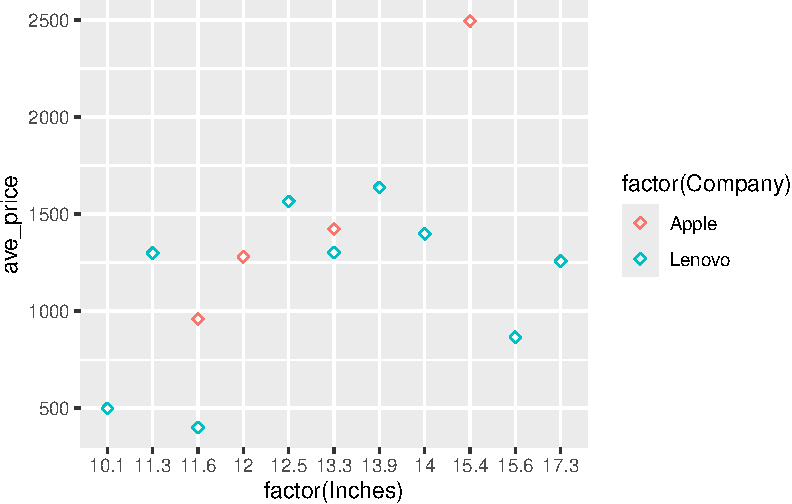
\includegraphics[keepaspectratio]{color_and_shapes_files/figure-pdf/fig-changingshapes-1.pdf}}

}

\caption{\label{fig-changingshapes}A \texttt{geom\_point()} with a
non-default shape}

\end{figure}%




\end{document}
